\documentclass[]{beamer}
%\usepackage[MeX]{polski}
%\usepackage[cp1250]{inputenc}
\usepackage{polski}
\usepackage[utf8]{inputenc}
\beamersetaveragebackground{blue!10}
\usetheme{Warsaw}
\usecolortheme[rgb={0.1,0.5,0.7}]{structure}
\usepackage{beamerthemesplit}
\usepackage{multirow}
\usepackage{multicol}
\usepackage{array}
\usepackage{graphicx}
\usepackage{enumerate}
\usepackage{amsmath} %pakiet matematyczny
\usepackage{amssymb} %pakiet dodatkowych symboli

\title{Philip Anthony Hopkins}
\date{
Data i miejsce urodzenia: 31 grudnia 1937 (79 lat)
Port Talbot, Walia, Wielka Brytania}
{
\begin{figure}
\begin{center}
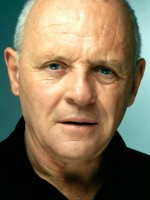
\includegraphics[scale=0.2]{hopkins.jpg}
\end{center}
\end{figure}
}
\begin{document}
\frame
{
\maketitle
}
\frame
{
\frametitle{Życiorys}
Uważany jest za jednego z najwybitniejszych aktorów współczesnych, potrafiącego zagrać role w szerokim spektrum gatunków filmowych i teatralnych. W młodości miał na niego wielki wpływ Richard Burton, którego poznał osobiście mając 15 lat. Według krytyków obie postacie aktorów były bardzo podobne zarówno fizycznie, pod względem temperamentu jak i stylu gry aktorskiej. Początkowo jego aktorska kariera zawodowa opierała się wyłącznie na rolach teatralnych. W późniejszym okresie skupił się na aktorstwie filmowym. Jego najsławniejszą rolą filmową była postać Hannibala Lectera w filmie Milczenie owiec, za którą otrzymał w 1992 nagrodę Oscara Amerykańskiej Akademii Filmowej za najlepszą rolę męską. Grał także w sequelu Hannibal (2001) oraz w prequelu Czerwony smok (2002). Zamieszkał w Stanach Zjednoczonych, a od 2000 posiada obywatelstwo tego kraju. Był trzykrotnie żonaty. W 2002 zakończył 29-letni związek małżeński z Jennifer Lynton i ożenił się w 2003 ze Stellą Arroyave.
}
{
\begin{center}
	\begin{tabular}{ | 1 | 1 | p{5cm} |}
	\hline
Film  &  Rola & Reżyser \\ \hline
Milczenie owiec(1991) & Dr Hannibal Lecter & Jonathan Demme \\ \hline
Okruchy dnia(1993)& James Stevens & James Ivory \\ \hline
Hannibal(2001) & Dr Hannibal Lecter & Ridley Scott \\ \hline
Człowiek słoń (1980) & Dr Frederick Treves & David Lynch \\ \hline
Prawdziwa historia (2005) & Burt Munro & Roger Donaldson \\ \hline
Czerwony smok (2002) & Dr hannibal lecter & brett ratner \\ \hline
\hline
\end{tabular}
\end{center}
}

\begin{block}
{Ciekawostki bardziej i mniej znane o Antku}
W 1957 roku ukończył Royal Welsh College of Music & Drama w Cardiff (Walia, Wielka Brytania). Jest doktorem honoris causa Uniwersytetu Walijskiego. Tytuł nadano mu w 1988 roku.
W 1987 roku otrzymał Order Komandorski Imperium Brytyjskiego. 
W 2000 roku otrzymał obywatelstwo amerykańskie, zachowując jednak tytuł "Sir" nadany mu w 1993 roku w Anglii.Oferowano mu rolę w filmie "Nieustraszeni bracia Grimm". Na początku propozycję przyjął, później jednak zrezygnował z udziału przy produkcji obrazu.W 2012 roku wydał debiutancką płytę pt. "Composer". 
Podczas kręcenia filmu "Lekcja przetrwania" otarł się o śmierć, wpadając do rzeki. Efektem była hipotermia i pobyt w szpitalu.
\end{block}
{
\begin{figure}[1]
\begin{center}
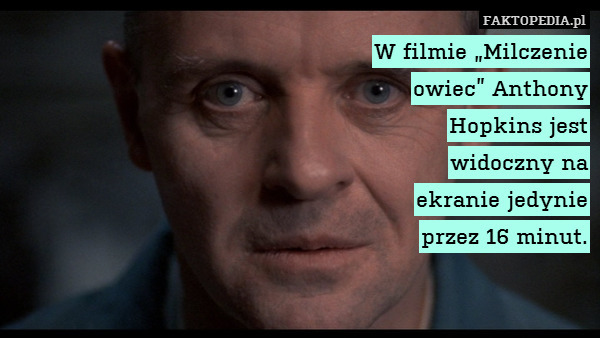
\includegraphics[scale=0.5]{ciekawostka.jpg}
\end{center}
\end{figure}
}
\begin{alertblock}
{Warto zapamiętać:}
31 grudnia 1937 - 3 listopada 2017
Aktor dalej żyje i ma się dobrze!
\end{alertblock}
}
\frame
{
\frametitle{Nagrody}
Wielokrotnie nominowany, również laureat m.in:
\begin{itemize}
	\item <1-6> Nominacja Oscar -za Najlepszy aktor drugoplanowy za film Amistad (1997)
	\item <2-6> Nominacja Oscar	-Najlepszy aktor pierwszoplanowy za film Nixon (1995)
	\item <3-6> Nominacja Oscar -Najlepszy aktor pierwszoplanowy za film Okruchy dnia (1993)
	\item <4-6> Laureat Oscara -Najlepszy aktor pierwszoplanowy za film Milczenie owiec (1991)
	\item <5-6> Nominacja Złoty Glob -Najlepszy aktor w dramacie za film Okruchy dnia (1993)
	\item <6-6>	Nominacja Złoty Glob -Najlepszy aktor w miniserialu lub filmie telewizyjnym za film Dziesiąty człowiek (1988)
\end{itemize}
}

\end{document}
